\chapter{Majorisation--Minimisation Preconditioners}
\label{app:mm_preconditioner}

Chapter~\ref{chapter:optimisation} builds its prior-curvature models from the Lewis--Sendov Hessian of \wdtnv. This appendix describes an alternative built from a quadratic majoriser of the prior. It is not used in Chapter~\ref{chapter:paper}, but its diagonal form was used for the subset experiment (Section~\ref{sec:optimisation_subset_selection}).

\section{Construction}

Let $Y,Y_0\in\mathbb{R}^{d\times M}$, let $\phi(Y)=\sum_{i}g(\sigma_i(Y))$ with $g$ the Charbonnier function of Chapter~\ref{chapter:wdtnv}, and let $C_0=\Omegaeps{Y_0}$. Then
\begin{equation}
    \phi(Y)
    \leq
    \phi(Y_0)
    +\tfrac12\operatorname{tr}\!\left[\left(Y^\top Y-Y_0^\top Y_0\right)C_0\right],
    \label{eq:jacobian_majoriser}
\end{equation}
with equality at $Y=Y_0$. Since $\phi(Y)=\operatorname{tr}((Y^\top Y+\epsilon^2\mathbb{I}_M)^{1/2})-M\epsilon$ and the matrix square root is operator concave \cite{bhatiaMatrixAnalysis1997a}, $\phi$ is a concave function of the Gram matrix $Y^\top Y$, and~\eqref{eq:jacobian_majoriser} is its tangent bound. For $M=1$, $C_0$ is the familiar \gls{irls} weight for the Charbonnier potential \cite{fessler_image_2017,charbonnier_deterministic_1997}. It is also the same inverse square root that evaluates the prior gradient in Chapter~\ref{chapter:wdtnv}.

Summing~\eqref{eq:jacobian_majoriser} over voxels, with $Y_0$ the weighted directional Jacobian $\tilde{\mathcal G}_n$ at a preconditioner refresh, gives a quadratic majoriser of the prior. Its Hessian couples neighbouring voxels, so, as for the Lewis--Sendov models, only voxel blocks are retained. Writing $C_r=\Omegaeps{\tilde{\mathcal G}_r}$ at target voxel $r$, the voxel block of this Hessian is
\begin{equation}
    \widehat H_{\mathcal R,n}^{\mathrm{MM\text{-}block}}
    =
    V_{\mathrm{vox}}
    \sum_{r\in\mathcal N(n)}
    \left[B_rC_rB_r\right]\circ A_{r\leftarrow n},
    \qquad
    [A_{r\leftarrow n}]_{mm'}
    =
    c_{r\leftarrow n}^\top\Pi_{m,r}^\top\Pi_{m',r}c_{r\leftarrow n},
    \label{eq:mm_block_preconditioner}
\end{equation}
where $\mathcal N(n)$ is the set of target voxels whose finite-difference stencil contains $n$, $c_{r\leftarrow n}$ is the response at $r$ of the difference operator to a unit impulse at $n$, $B_r=\operatorname{diag}(\rho_{1,r},\rho_{2,r})$, and $\circ$ is the Hadamard product. The \emph{Jacobi diagonal} keeps the diagonal of each block.

If valid data and prior majorisers are built at a common anchor, their curvatures add, and the inverse sum~\eqref{eq:parallel_sum_combination} is the corresponding \gls{mm} step. Extracting voxel blocks or diagonals from the spatially coupled Hessian does not preserve the majorisation, however, so none of these models is a global majoriser and the interpretation is heuristic.

\section{Cost and Comparison}

Construction and cached application of the two block models were timed on an NVIDIA RTX 3080 using ten repeats after two warm-up evaluations, for the one-bed phantom and two-bed patient configurations (Table~\ref{tab:mm_preconditioner_cost}). Application costs the same for both, but \gls{mm} construction is cheaper: Lewis--Sendov construction took 51\% and 72\% longer for one and two beds. This reflects the work each needs: the \gls{mm} block needs only the $2\times2$ inverse square root $C_r$ at each target, whereas the Lewis--Sendov block needs voxel-wise singular-value decompositions and the spectral Hessian terms built from them. Using the Chapter~\ref{chapter:paper} subset counts (18 PET plus 12 SPECT for one bed, or 36 PET plus 12 SPECT for two beds), with one construction and 30 or 48 applications per epoch, application dominates and the saving is small: approximately $8.2$ versus $8.5\,\mathrm{s}$ per epoch for one bed, and $55.7$ versus $58.3\,\mathrm{s}$ for two beds.

\begin{table}[htbp]
    \centering
    \caption{Mean construction and cached application times in seconds for the two block preconditioners; uncertainties are standard deviations over ten repeats.}
    \label{tab:mm_preconditioner_cost}
    \small
    \begin{tabular}{@{}llrr@{}}
        \toprule
        Preconditioner & Operation & One bed & Two beds\\
        \midrule
        \multirow{2}{*}{\gls{mm} block}
            & Construction & $0.920 \pm 0.0149$ & $3.416 \pm 0.0259$\\
            & Application  & $0.242 \pm 0.0019$ & $1.090 \pm 0.0046$\\
        \addlinespace
        \multirow{2}{*}{Lewis--Sendov block}
            & Construction & $1.389 \pm 0.0141$ & $5.867 \pm 0.0395$\\
            & Application  & $0.237 \pm 0.0011$ & $1.093 \pm 0.0052$\\
        \bottomrule
    \end{tabular}
\end{table}

\begin{figure}[htbp]
    \centering
    \begin{subfigure}{0.99\linewidth}
        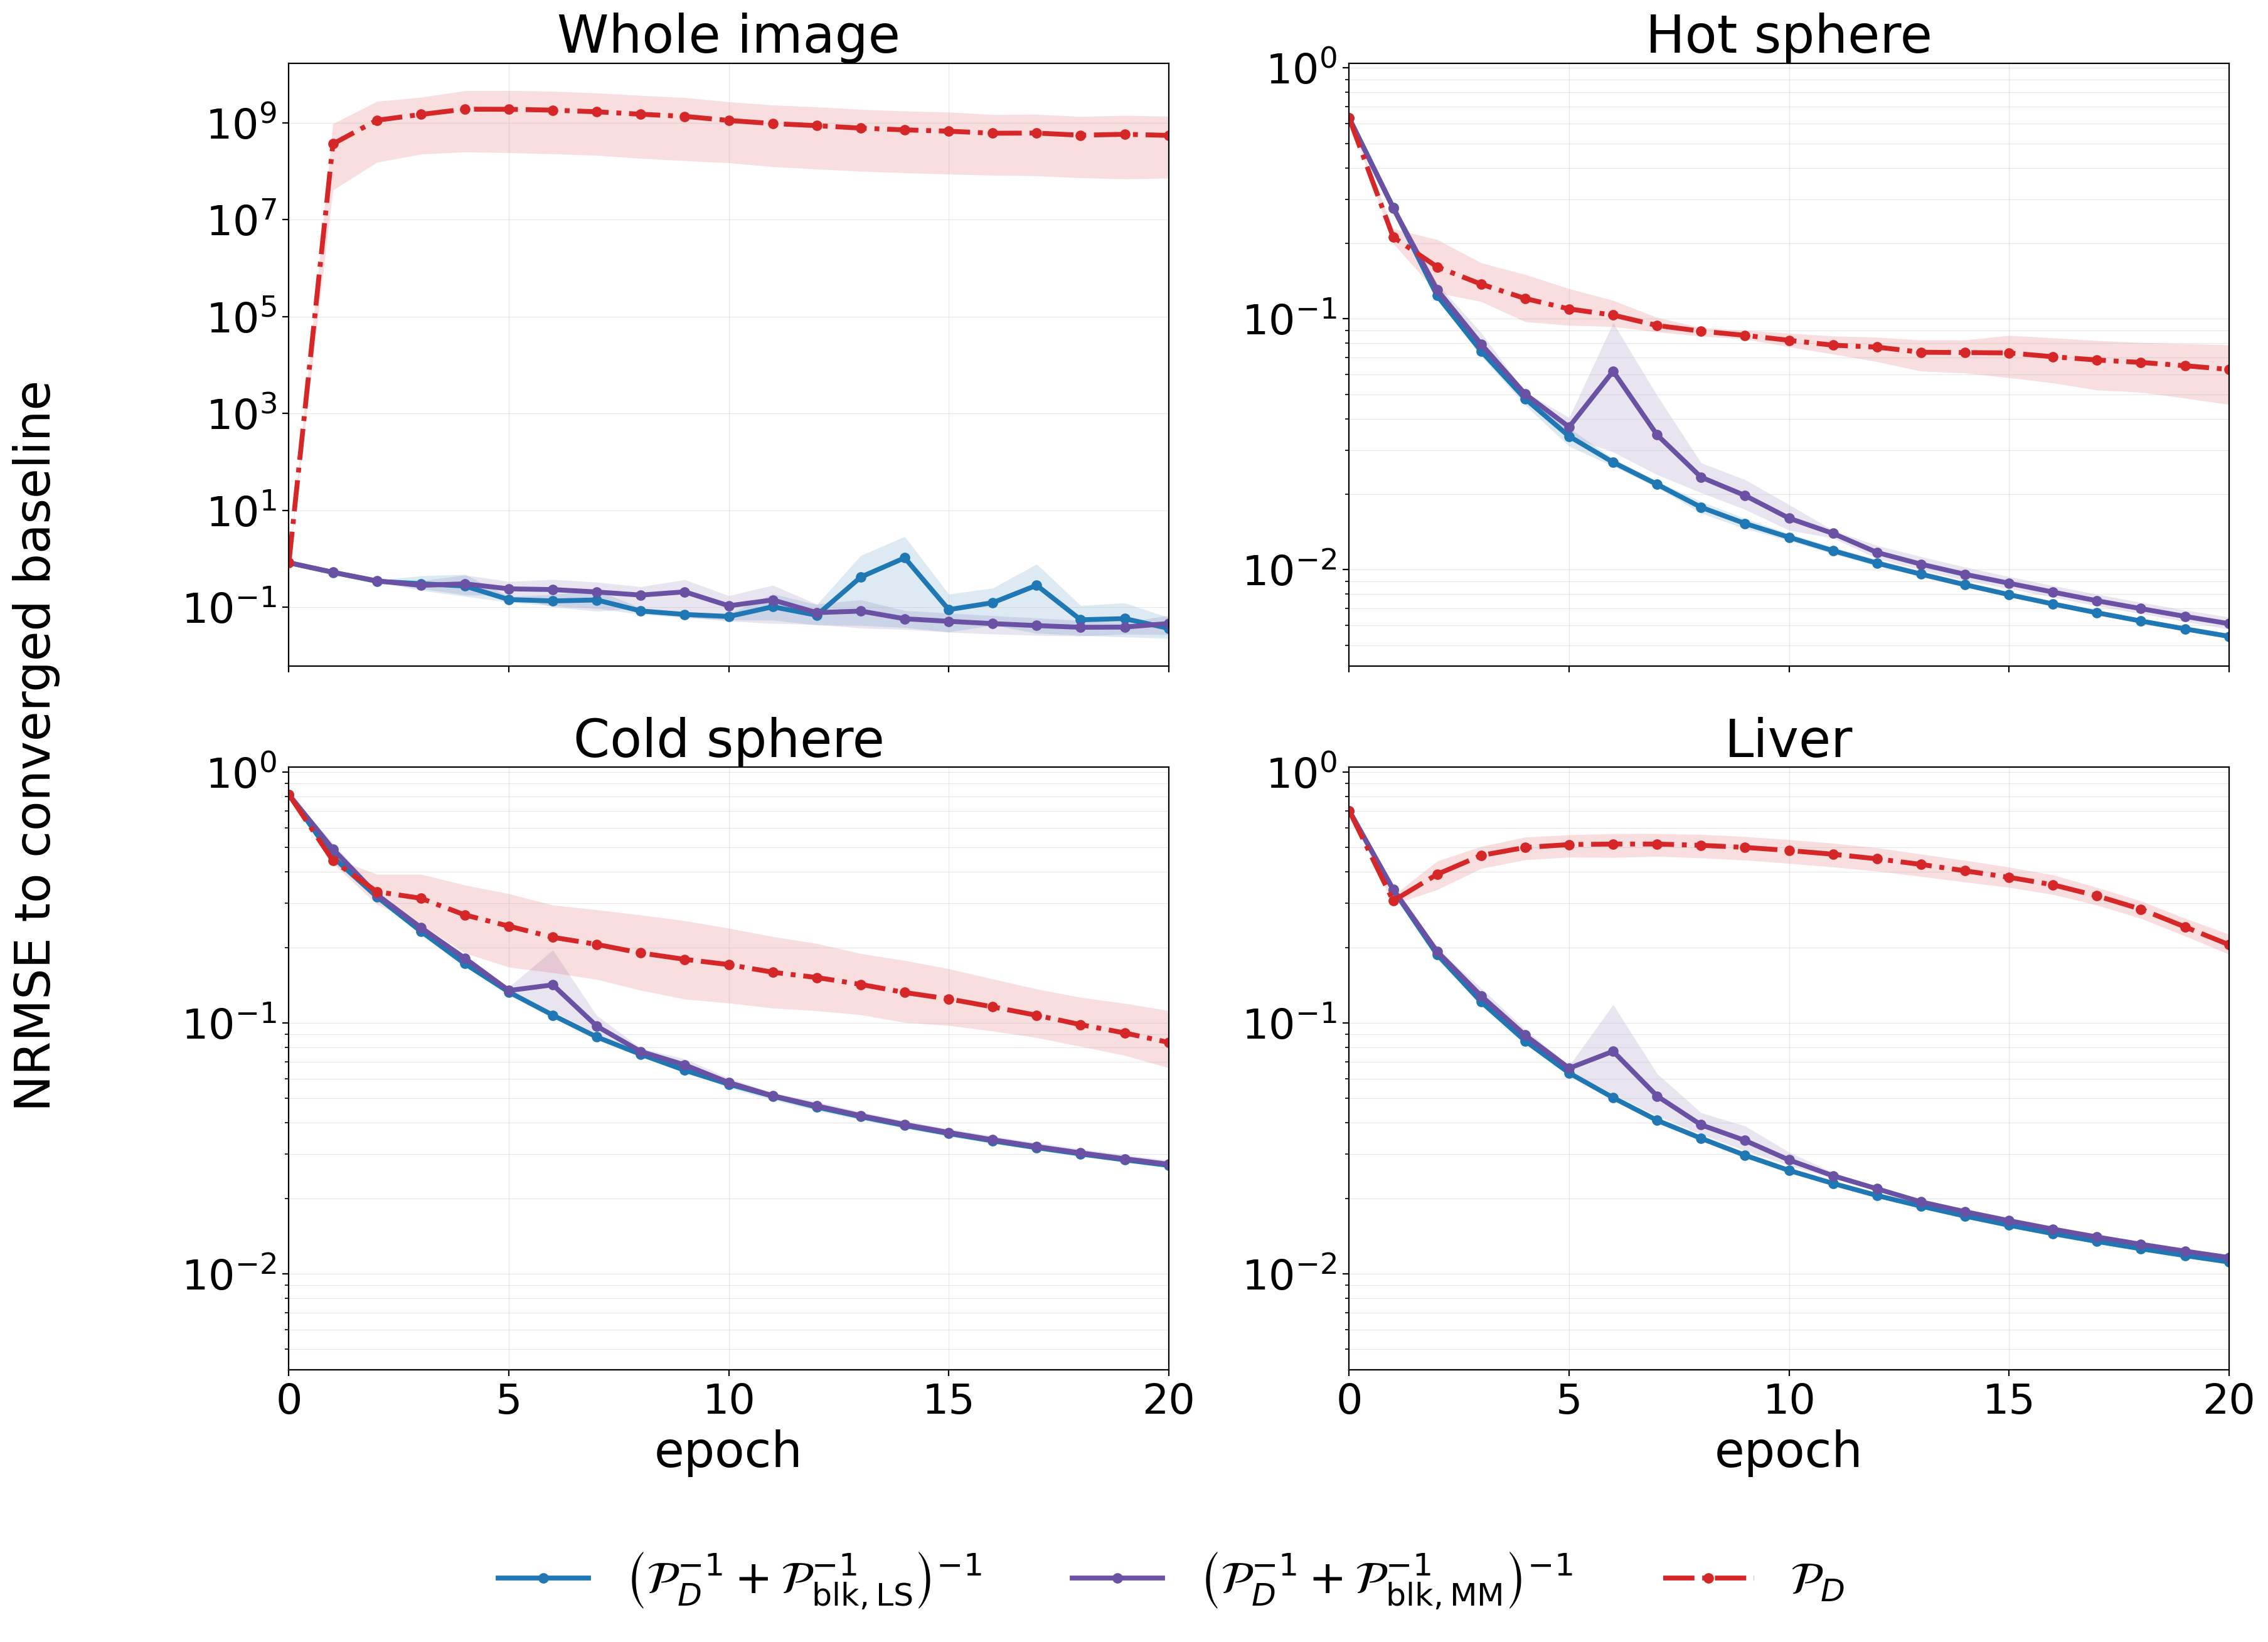
\includegraphics[width=\linewidth]{figures/preconditioning/ls_vs_mm_blk/exp3_best_precond_1bpos.png}
        \caption{\gls{pet}.}
    \end{subfigure}
    \begin{subfigure}{0.99\linewidth}
        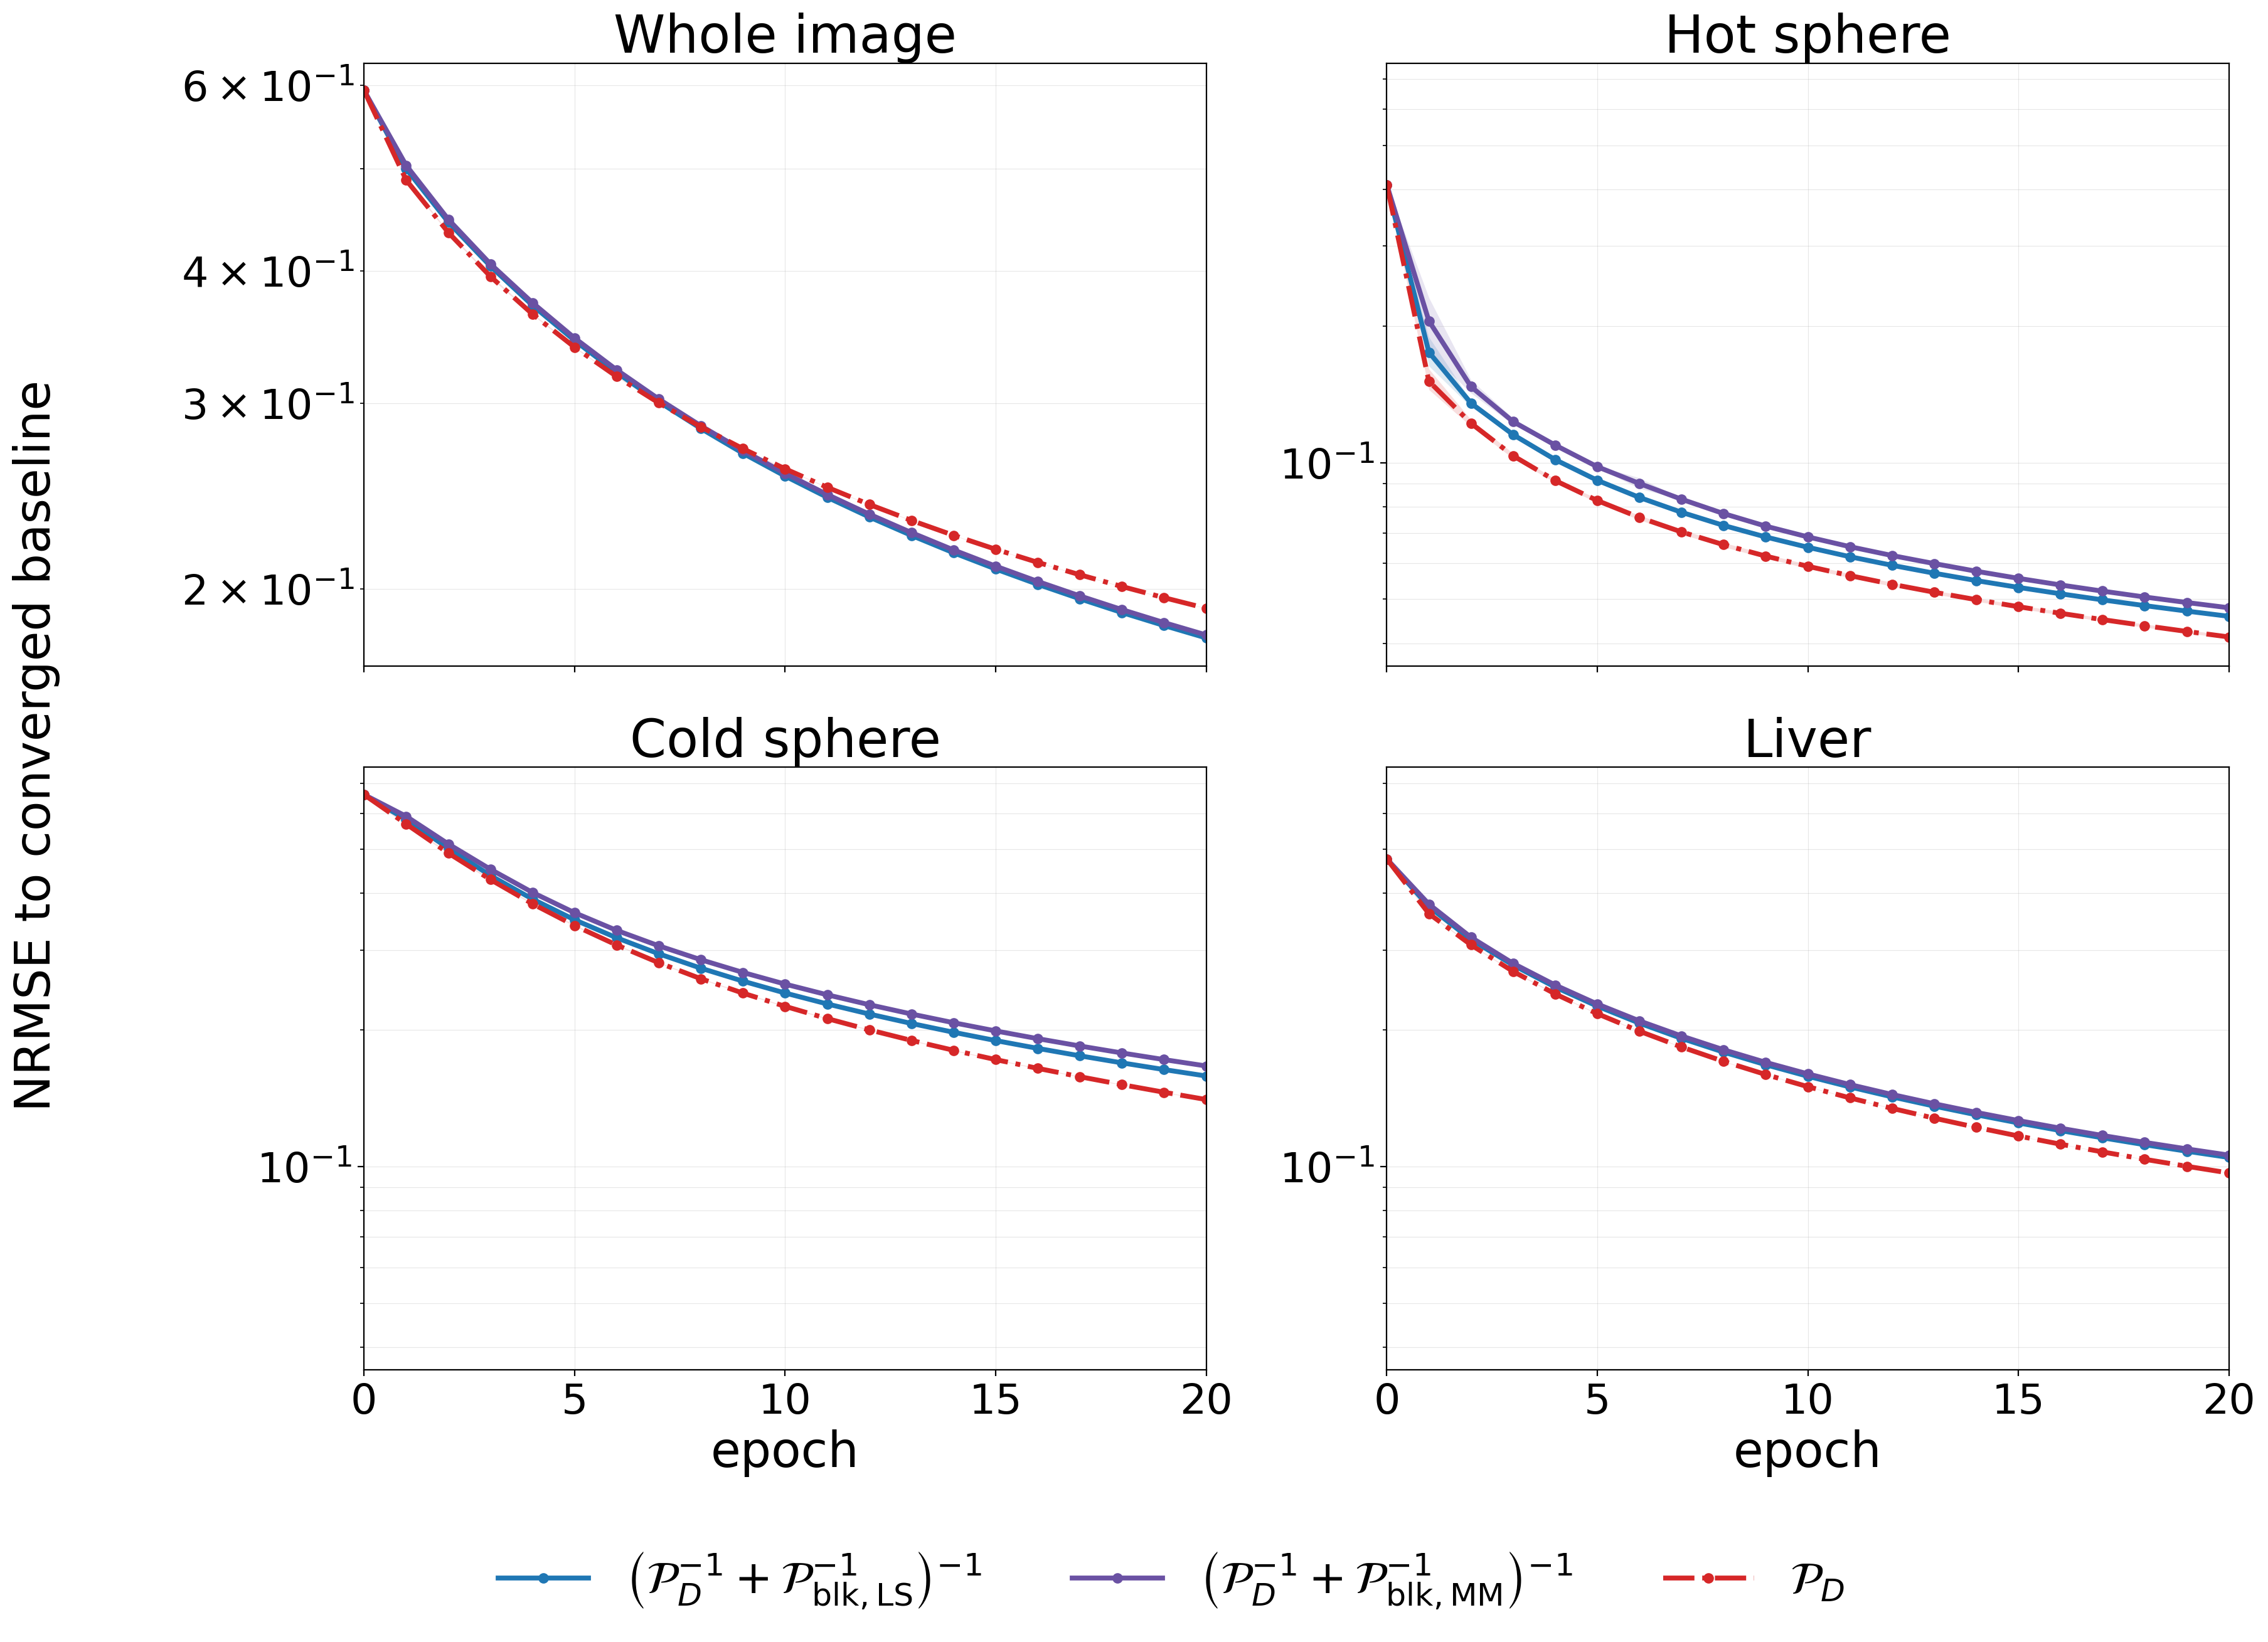
\includegraphics[width=\linewidth]{figures/preconditioning/ls_vs_mm_blk/exp3_best_precond_1bpos_SPECT.png}
        \caption{\gls{spect}.}
    \end{subfigure}
    \caption{\gls{nrmse} trajectories for the inverse-sum combinations of data-only scaling with the Lewis--Sendov ($\mathcal P_{\mathrm{blk,LS}}$) and \gls{mm} ($\mathcal P_{\mathrm{blk,MM}}$) block prior models, with data-only \gls{bsrem} ($\mathcal P_D$) for reference. Lines and shading show the five-run mean and pointwise minimum--maximum over 20 matched expected data-draw units.}
    \label{fig:mm_vs_ls_block}
\end{figure}

Under the protocol of Section~\ref{subsec:preconditioner_experiment_methods}, the two block models gave similar \gls{nrmse} (Figure~\ref{fig:mm_vs_ls_block}). The Lewis--Sendov block was slightly lower in most anatomical regions. The \gls{mm} block showed a transient increase near pass 6 in the \gls{pet} anatomical regions, and the Lewis--Sendov block showed transient whole-image increases near passes 14 and 17. With similar convergence and cheaper construction, the \gls{mm} block is a reasonable alternative where construction cost matters.
